\chapter{把握环境控制过程}
\section{把握组织环境}
\subsection{组织环境的概念}
组织:人类通过社会活动,按照一定目的、任务和形式加以编制的群体。
\par \textbf{组织环境:}存在于组织外部,和组织密切联系,决定组织存在和发展的自然、经济、技术、政治、社会的各种因素和条件的集合体。
\par 组织环境:自然环境和社会环境。
\par 组织环境对IT项目的效益和效率起关键作用,是IT项目管理的基础。
\subsection{组织环境的特征}
\begin{itemize}
	\item \textbf{客观性:} 组织环境是客观存在的,它不随组织中人们的主观意志为转移,它制约着组织的活动。
	\item \textbf{系统性: }组织环境是由与组织相关的各种外部事物和条件相互有机联系所组成的整体,组织的外部环境和内部环境构成了不同层次的子系统。项目的管理活动是在这种整体性的环境背景中进行的。
	\item \textbf{动态性:}组织环境的各种因素是不断变化的,各种组织环境因素又在不断地重新组合,不断形成新的组织环境。 
\end{itemize}
\subsection{战略计划与项目的选择}
IT项目人员应该将对组织战略计划的理解放在首要位置。
\par \textbf{战略:}是指战争中整体性、长期性、基本性问题的计谋。
\par 战略和战术区别:
\begin{itemize}
	\item 战略针对整体性问题,战术针对局部性问题;
	\item 战略针对长期性问题,战术针对短期性问题;
	\item 战略针对基本性问题,战术针对具体性问题。
\end{itemize}
\par \textbf{战略计划:}通过对组织优势、劣势的分析,研究组织环境中存在的机会与挑战,预测未来的趋势,展望新的产品和服务需求,从而确定的长远目标规划。
\par 人们将组织的整体性、长期性、基本性计划称为战略计划。
\par \textbf{IT项目计划:}确定IT战略计划、分析业务、编制项目计划和项目资源分配。
\par SWOT分析(战略计划分析)将与研究对象密切相关的各种内部优势因素(Strengths)、弱点因素(Weaknesses)、机会因素(Opportunities)和威胁(Threats) 因素,通过调查分析和罗列后按矩阵形式排列,并运用系统分析的原理,将各种因素相互匹配加以分析,从中得出一系列相应的结论。
\par 核心问题:强项、弱项、机会、威胁因素。
\par SWOT分析实质:核心竟争力的分析。
\par \textbf{IT项目计划的核心目标:}建立组织的信息战略。
\par 其他关键词:“战略信息系统”、投资IT项目原因。
\section{掌握系统方法}
\subsection{系统的定义}
系统(system):由\textbf{相互联系和相互制约}(一定的结构)的\textbf{若干组成部分结合}成的、具有\textbf{特定功能}的有机整体。
\subsection{系统的特征}
\begin{enumerate}
	\item 集合性是系统最基本的特征
	\item 系统的结构是有层次的
	\item 系统具有相关性
\end{enumerate}
\subsection{系统的原理}
系统原理为认识项目管理的本质和方法提供了新的视角,主要体现在:
\begin{itemize}
	\item 整体性原理
	\item 动态性原理
	\item 开放性原理
	\item 环境的适应性原理
	\item 综合性原理
\end{itemize}
\subsection{系统方法}
\begin{itemize}
	\item 以系统的方法从整体的视角看待项目和项目运营的组织环境;
	\item 用系统思维对项目的成功具有关键的作用;
	\item 系统方法是解决复杂问题的一个整体方法,包括\underline{系统观念、系统分析和系统管理}。
\end{itemize}
\subsubsection*{系统观念}
系统观念是指一整套系统地思考事物的思维模式。
\begin{itemize}
	\item 任何事物都是作为系统而存在的,都按照一定结构组成有机整体;
	\item 系统思维要求要整体系统看,也要分开辩证看;
	\item 从整体的角度把系统中的各种因素进行协调和处理,以求达到对问题做出最佳地处理。
\end{itemize}
\subsubsection*{系统分析}
系统分析是一种解决问题的方法。
\begin{itemize}
	\item 通过确定系统的研究范围,将其分解为各个组成要素;
	\item 然后识别和评价各要素存在的问题、机会、约束、需求;
	\item 对提出的解决方案站在系统的高度进行比较,筛选一个最优的方案。
\end{itemize}
\subsubsection*{系统管理}
系统管理是在一个系统进行变革的过程中,运用系统的原理来管理和解决相关的问题。
\par \textbf{项目经理的基本要求和系统管理的首要任务:}明确IT项目的关键业务、技术和组织以及各个项目间的相关性。
\section{熟悉项目阶段}
\subsection{项目阶段性特征}
项目成功的三大支柱:项目的范围、工期和团队规模。
\par 项目划分原因:简化项目的复杂度和可控性,更好的处理项目与组织的日常运营之间的关系,提高项目的成功率。
\par 项目阶段的划分:定义、开发、实施和收尾。
\par \textbf{项目可行性阶段:}项目定义阶段和开发阶段的主要工作是形成项目计划。
\par \textbf{项目获取阶段:}项目实施阶段和收尾阶段的主要工作是根据项目计划开展实际工作。
\begin{itemize}
	\item 定义阶段:制定项目建议书;
	\item 开发阶段:规划项目,指定详细项目计划;
	\item 实施阶段:执行项目计划,并进行项目的监督和控制;
	\item 收尾阶段:完成项目的验收与工作总结,为后续的项目提供经验、教训和帮助。
\end{itemize}
阶段评审目的:
\begin{itemize}
	\item 一是决定该项目是否可以进入下一个阶段;
	\item 二是尽可能以较小的代价查明和纠正错误。
\end{itemize}
\subsection{项目的生命周期}
\begin{figure}[!h]
	\centering
	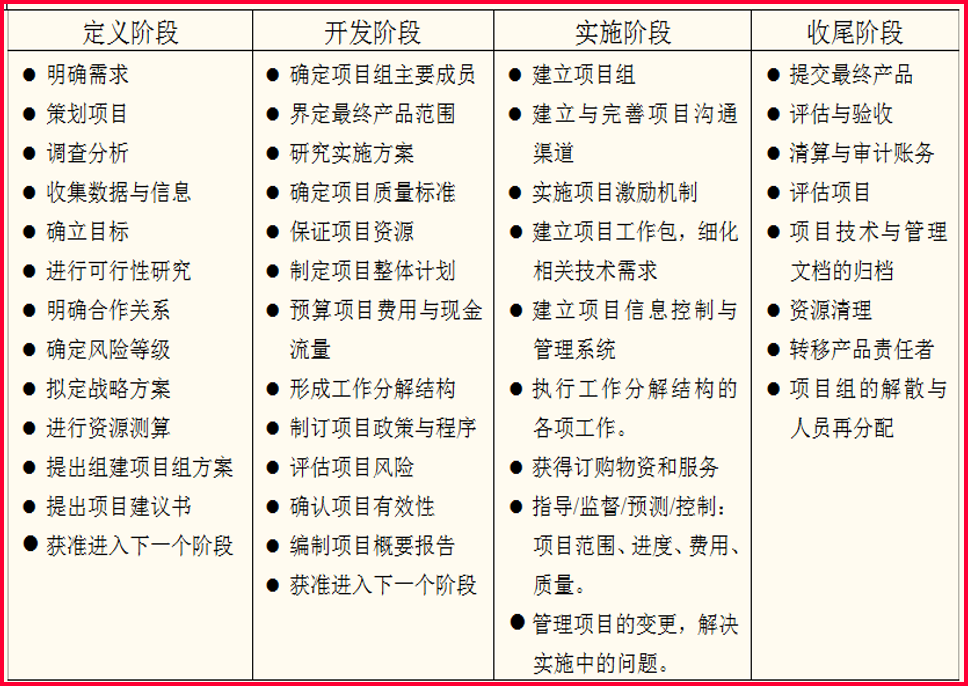
\includegraphics[width=0.8\textwidth]{image/2-1}
	\caption{项目的生命周期及其主要工作}
\end{figure}
\begin{itemize}
	\item 对于开发商,开始:与客户签订开发合同,结束:完成合同规定的任务。
	\item 对于客户,开始:需求的提出,结束:使用项目产品实现目标。
\end{itemize}
\par 站在客户的角度有利于成功。
\par IT项目的生命周期:识别需求、确定方案、执行项目、结束项目。
\subsection{软件产品生命周期与项目生命周期的关系}
软件产品的生命周期包括产品项目筛选、概念形成、产品开发、产品上市、市场增长、成熟和衰退直到退出市场为止。
\begin{itemize}
	\item 软件产品的生命周期从提出软件产品研发开始,直到最后停止使用该软件产品为止;
	\item 对于软件企业来说,产品的市场成功才是开发项目结束的真正标志。
\end{itemize}
\begin{figure}[!h]
	\centering
	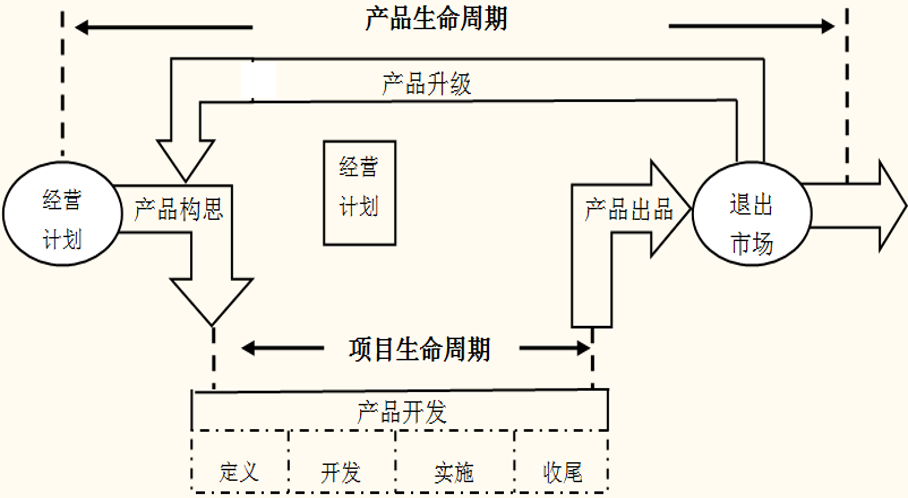
\includegraphics[width=0.8\textwidth]{image/2-2}
	\caption{项目生命周期与产品生命周期的关系}
\end{figure}
\section{了解项目组织}
\subsection{组织的定义与形成过程}
项目管理与传统组织管理的最大区别:项目管理更强调项目经理的作用,强调团队的协作精神,其组织形式具有更大的灵活性和柔性。
\par 项目组织是所有活动的焦点。
\par 组织的定义:
\begin{itemize}
	\item (名词)是指有意识形成的职务或职位的结构;
	\item (动词)是指为了达到某种目的而设计组织结构的工作过程。
\end{itemize}
\subsection{组织的特征}
组织的特征:目的性、专业化分工、依赖性、等级制度、开放性、环境的适应性。
\par 组织的原则:目标一致性、合理的管理幅度和层次、命令统一、责任与权力对等、合理分工与密切协作、集权与分权相结合、环境适应性。
\subsection{项目的组织结构}
与项目有关的组织结构:
\begin{itemize}
	\item 职能型
	\item 项目型
	\item 矩阵型:弱矩阵、平衡矩阵、强矩阵
\end{itemize}
\begin{figure}[!h]
	\centering
	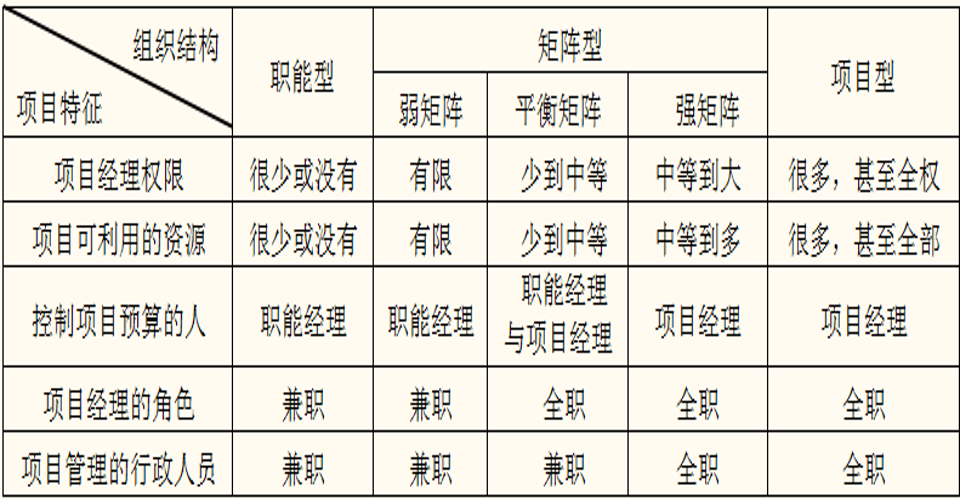
\includegraphics[width=0.8\textwidth]{image/2-3}
	\caption{组织结构对项目和项目经理的影响}
\end{figure}
\subsection{组织文化对项目组织的影响}
管理之魂的组织文化:协调力和凝合剂。
\par 组织文化:组织在长期的实践活动中所形成的并且为组织成员普遍认可和遵循的具有本组织特色的价值观念、团体意识、行为规范和思维模式的总和。
\par 组织文化的任务:努力创造这些共同的价值观念体系和共同的行为准则。
\subsection{IT项目组织的特点}
\begin{itemize}
	\item 客户适应性
	\item 任务导向性
	\item 利益冲突性
	\item 组织动态性
	\item 责权的不对称性
	\item 信息的不对称性
	\item 全过程的风险性
\end{itemize}
\section{控制项目过程}
活动的作用:
\begin{itemize}
	\item 人作用于物的活动,这涉及到有关操作的知识;
	\item 人作用于人的活动,这涉及到有关协调的知识。
\end{itemize}
项目的过程分为两类:
\begin{itemize}
	\item 一类是产品导向型过程,它注重对项目产品进行具体说明并进行制造(通过项目生命周期定义)。
	\item 另一类是项目管理过程,它注重对项目工作进行描述和组织,项目管理的过程在大多数时候对多数项目都是适用的。
\end{itemize}
\subsection{项目管理过程组}
项目管理过程:启动、规划、执行、监督和结束。
\begin{figure}[!h]
	\centering
	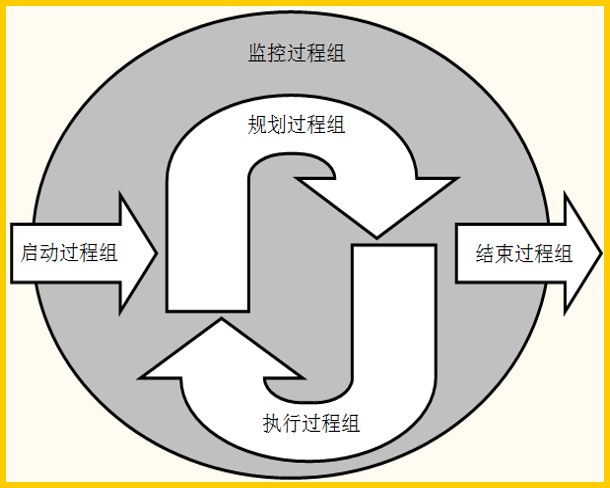
\includegraphics[width=0.5\textwidth]{image/2-4}
	\caption{项目管理过程组}
\end{figure}
\begin{figure}[!h]
	\centering
	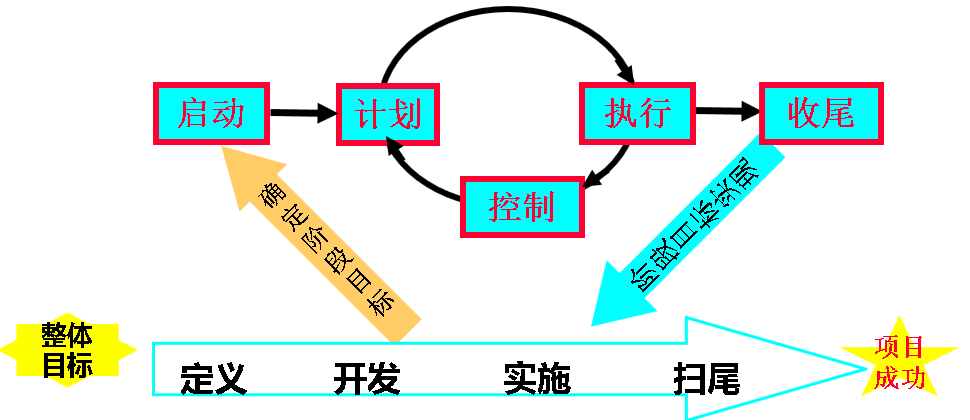
\includegraphics[width=0.6\textwidth]{image/2-5}
	\caption{项目管理过程组之间关系}
\end{figure}
\subsubsection*{启动过程组}
主要任务:确定并核准项目或项目阶段;
\par 主要成果:形成一个项目章程和选择一位项目经理。
\subsubsection*{规划过程组}
主要任务:确定和细化目标,并规划为实现项目目标和项目范围的行动方针和路线,确保实现项目目标;
\par 主要成果:包括完成工作任务分解结构、项目进度计划和项目预算。
\subsubsection*{执行过程组}
主要任务:通过采用必要的行动,协调协调人力资源和其他资源,整体的、有效的实施项目计划
\par 主要成果:交付实际的项目工作。
\subsubsection*{监控过程组}
主要任务:定期测量和实时监控项目进展情况,发现偏离项目管理计划之处,及时采取纠正措施和变更控制,确保项目目标的实现;
\par 主要成果:在要求的时间、成本和质量限制范围内获得满意的结果。
\subsubsection*{收尾过程组}
主要任务:采取正式的方式对项目成果、项目产品、项目阶段进行验收,确保项目或项目阶段有条不紊的结束;
\par 主要成果:包括项目的正式验收、项目审计报告和项目总结报告编制以及项目组成员的妥善安置。
\subsection{启动过程组}
项目启动是识别和开始一个新项目或新阶段的过程,项目启动过程组由一组有助于正式授权开始一个新项目或一个项目阶段的过程组成。
\par 项目经理应该对这些文件进行消化、分析和归档,并明确项目与组织战略计划的关系以及组织内高层管理人员的责任。
\par 注:在项目定义阶段,启动过程一般由超出项目控制范围之外的组织、项目集或项目组合过程来完成。
\par 外部因素:事业环境因素、组织过程资产和项目发起人。
\par 启动过程:制定项目章程和制定项目初步范围说明书。
\par 启动原则:
\begin{itemize}
	\item 不但要明确能够做哪些事情,还有明确不能做哪些事情;
	\item 不但要明确完成的任务,还有明确完成这些任务的约束条件和验收标准;
	\item 不但要关注需要获得的成果,还要关注采用哪样的过程来获得这些成果。
\end{itemize}
\subsection{规划过程组}
规划过程组的重要工作:收集不完整和把握程度不一的各种信息。
\par 其他关键词:21个项目管理过程。
\subsection{执行过程组}
关键词:7个项目管理过程。
\par 首要问题:如何有效的获取、利用和管理资源。
\subsection{监控过程组}
任务:确保项目目标的实现。
\par 监控过程工作体现在两个方面:
\begin{itemize}
	\item 对照项目管理计划和项目实施基准来严格监视正在进行的项目活动;
	\item 对妨碍整体变更控制的因素施加影响,以确保项目成员仅实施经过批准的变更。
\end{itemize}
\par 项目有效控制的基础:里程碑。项目以目标来驱动。
\par 注:监控的是过程,而不是结果。关键词:12个项目管理过程。
\subsection{收尾过程组}
收尾过程组包括项目收尾和合同收尾2个过程。
\subsection{过程组之间的关系}
\begin{enumerate}
	\item 项目管理过程不是孤立的、一次性的活动;
	\item 贯穿始末,相互重叠;
	\item 项目阶段内的5个过程组是相互联系在一起的,一个过程组的成果或输出是另一个过程组的依据或输入。
\end{enumerate}
\begin{figure}[!h]
	\centering
	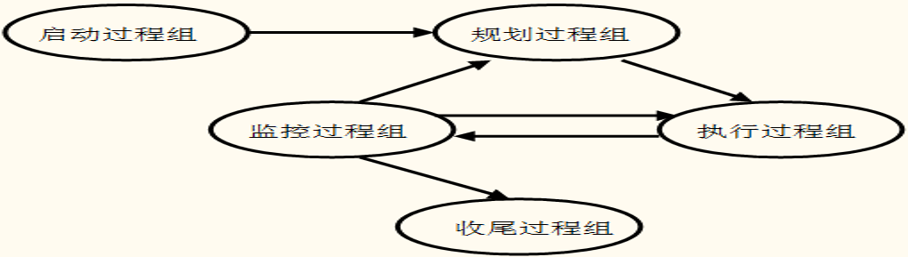
\includegraphics[width=0.6\textwidth]{image/2-6}
	\caption{项目管理过程组之间的关系 }
\end{figure}